\lecture{2024-04-04}{}
Let $(Z_t)_{t \in \N}$ be a Markov chain with state space
$S = \set{s_1, \dots, s_n}$ and transition matrix
$A = (a_{ij})_{i,j=1}^n$.
That is, \[
    \Pr(Z_{t+1} = s_j \given Z_t = s_i) = a_{ij}.
\]

If $Z_0 \sim \mu^\top$, then the distribution of $Z_n$ is $\mu^\top A^n$.

The Ising model is incredibly hard to compute.
Instead of computing \[
    \E[S_i] = \sum_s s_i \Pr(S = s),
\] we can sample \[
    \E[S_i] \approx \frac1m \sum_{i=1}^m s_i^*,
\] where $s_i^*$s are sampled according to the distribution
$\Pr(S = \cdot)$.

This is done via the Metropolis algorithm.

\chapter{Graphical Models} \label{chp:graph_models}
Let $\set{X_i}_{i=1}^d$ be a set of random variables.
To each $X_i$ assign a vertex $i$, and let the vertex set be $[d]$.
Edges will model dependencies between the random variables.

We first review some definitions from graph theory.
\section{Definitions} \label{sec:graph_def}
\begin{definition}
    A \emph{graph} $G = (V, E)$ consists of a set of vertices $V$
    and a set of edges $E \subseteq V \times V$.

    A graph is \emph{undirected} if $(u, v) \in E$ implies $(v, u) \in E$.
    Otherwise, it is \emph{directed}.

    A vertex $v$ is \emph{adjacent} to $u$ if $(u, v) \in E$.
    $u$ is said to be the \emph{parent} of $v$.

    The \emph{neighbourhood} of $v$ is the set of vertices adjacent to $v$.
    \[
        N(v) = \set{u \in V \given (u, v) \in E}.
    \]
\end{definition}

\begin{definition}[Paths] \label{def:graph:paths}
    A \emph{path} in a graph $G = (V, E)$ is a sequence of vertices
    $(v_1, \dots, v_k)$ such that $(v_i, v_{i+1}) \in E$ for all $i$.

    A path is \emph{simple} if all vertices are distinct.
    A path is \emph{closed} if $v_1 = v_k$.

    A \emph{cycle} is a closed path with no repeated vertices (except
    for the first and last).
\end{definition}

\begin{definition*}[Separation] \label{def:graph:separation}
    Let $A, B, C \subseteq V$ be disjoint.
    $A$ and $B$ are \emph{separated} by $C$ if every path from $A$ to $B$
    contains a vertex in $C$.
\end{definition*}

We now study two instances of graphical models:
\begin{itemize}
    \item Bayesian networks
    \item Markov networks
\end{itemize}
\subsection{Bayesian Networks} \label{sec:bayes_networks}
\begin{definition*}
    Let $G = ([n], E)$ be a directed acyclic graph.
    Then $(G, X_1, \dots, X_n)$ is a \emph{Bayesian network} if \[
        P(X_1=x_1, \dots, X_n=x_n)
            = \prod_{i=1}^n P(X_i \given \parent(i))
    \] where $\parent(i)$ is the set of parents of $i$.
\end{definition*}
For convenience, we will relabel the vertices in a topological sort.
Then for all $i$, \[
    \parent(i) \subseteq [i-1]
\]

\section{A real life example} \label{sec:bayes_networks:eg}
Let $N, T, L, X$ be random variables representing the following:
\begin{itemize}
    \item $N$ represents whether a particular patient has pneumonia.
    \item $T$ represents whether they have tuberculosis.
    \item $L$ represents whether they have observable lung abnormalities.
    \item $X$ represents whether they have a positive X-ray.
\end{itemize}
Then \begin{multline*}
    \Pr(N = n, T = t, L = l, X = x) \\
        = \Pr(N = n) \Pr(T = t)
        \Pr(L = l \given N = n, T = t)
        \Pr(X = x \given L = l).
\end{multline*} We will shorten such equations to \[
    \Pr(N, T, L, X) = \Pr(N) \Pr(T) \Pr(L \given N, T) \Pr(X \given L).
\] This can be represented by the following Bayesian network:
\begin{center}
    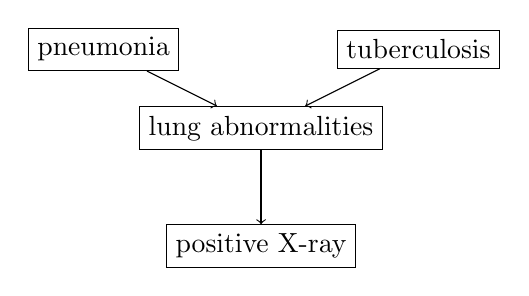
\begin{tikzpicture}
        \node[draw] (N) at (0, 0) {pneumonia};
        \node[draw] (T) at (4, 0) {tuberculosis};
        \node[draw] (L) at (2, -1) {lung abnormalities};
        \node[draw] (X) at (2, -2.5) {positive X-ray};

        \draw[->] (N) -- (L);
        \draw[->] (T) -- (L);
        \draw[->] (L) -- (X);
    \end{tikzpicture}
\end{center}
The \emph{inference problem} is to compute \[
    \Pr(N = 1 \given X = x).
\] Suppose the X-ray machines are awesome, so that $L=X$ with probability 1.

\subsection{HMMs} \label{sec:bayes_networks:hmms}
Consider the following Bayesian network:
\begin{center}
    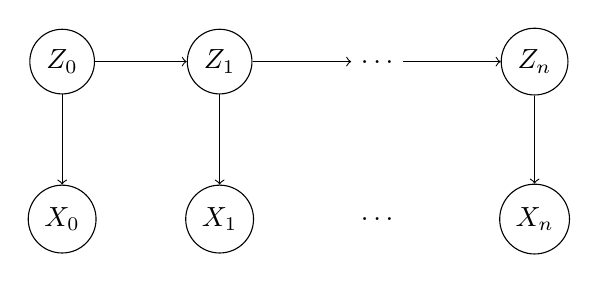
\begin{tikzpicture}[yscale=2]
        \node[draw, circle] (Z0) at (0, 0) {$Z_0$};
        \node[draw, circle] (Z1) at (2, 0) {$Z_1$};
        \node               (Zs) at (4, 0) {$\dots$};
        \node[draw, circle] (Zn) at (6, 0) {$Z_n$};
        \node[draw, circle] (X0) at (0, -1) {$X_0$};
        \node[draw, circle] (X1) at (2, -1) {$X_1$};
        \node               (Xs) at (4, -1) {$\dots$};
        \node[draw, circle] (Xn) at (6, -1) {$X_n$};

        \path[->]
            (Z0) edge (Z1) edge (X0)
            (Z1) edge (Zs) edge (X1)
            (Zs) edge (Zn)
            (Zn) edge (Xn);
    \end{tikzpicture}
\end{center}
The total probability is \[
    \Pr(X_0, Z_0, \dots, X_n, Z_n)
        = \Pr(Z_0)
            \prod_{i=1}^n \Pr(Z_i \given Z_{i-1})
            \prod_{i=0}^n \Pr(X_i \given Z_i).
\] This is the hidden Markov model!

\section{Markov Networks} \label{sec:markov_networks}
\begin{definition*}[Global Markov property] \label{def:markoc:gmp}
    Let $G = ([n], E)$ be undirected.
    Then $(G, X_1, \dots, X_n)$ satisfies the \emph{global Markov property}
    if for all $A, B, C \subseteq [n]$ such that $A$ and $B$ are separated
    by $C$, \[
        X_A \indep X_B \given X_C,
    \] where $X_S = \set{X_i}_{i \in S}$.
\end{definition*}

\begin{theorem}[Hammersly-Clifford theorem] \label{thm:markov_networks:hct}
    If $(G, X_1, \dots, X_n)$ satisfies the global Markov property,
    and $P(X_1, \dots, X_n) > 0$,
    then the joint distribution of $X_1, \dots, X_n$ factorizes over $G$.
    That is, \[
        \Pr(X_1, \dots, X_n)
            = \frac1Z \prod_{C \in \text{cliques}(G)} \psi_C(X_C),
    \] where $Z$ is a normalizing constant and $\psi_C$ is a potential
    function.
\end{theorem}
